\documentclass{beamer}

% xcolor and define colors -------------------------
\usepackage{xcolor}

% https://www.viget.com/articles/color-contrast/
\definecolor{purple}{HTML}{5601A4}
\definecolor{navy}{HTML}{0D3D56}
\definecolor{ruby}{HTML}{9a2515}
\definecolor{alice}{HTML}{107895}
\definecolor{daisy}{HTML}{EBC944}
\definecolor{coral}{HTML}{F26D21}
\definecolor{kelly}{HTML}{829356}
\definecolor{cranberry}{HTML}{E64173}
\definecolor{jet}{HTML}{131516}
\definecolor{asher}{HTML}{555F61}
\definecolor{slate}{HTML}{314F4F}

% Mixtape Sessions
\definecolor{picton-blue}{HTML}{00b7ff}
\definecolor{violet-red}{HTML}{ff3881}
\definecolor{sun}{HTML}{ffaf18}
\definecolor{electric-violet}{HTML}{871EFF}

% Main theme colors
\definecolor{accent}{HTML}{00b7ff}
\definecolor{accent2}{HTML}{871EFF}
\definecolor{gray100}{HTML}{f3f4f6}
\definecolor{gray800}{HTML}{1F292D}


% Beamer Options -------------------------------------

% Background
\setbeamercolor{background canvas}{bg = white}

% Change text margins
\setbeamersize{text margin left = 15pt, text margin right = 15pt} 

% \alert
\setbeamercolor{alerted text}{fg = accent2}

% Frame title
\setbeamercolor{frametitle}{bg = white, fg = jet}
\setbeamercolor{framesubtitle}{bg = white, fg = accent}
\setbeamerfont{framesubtitle}{size = \small, shape = \itshape}

% Block
\setbeamercolor{block title}{fg = white, bg = accent2}
\setbeamercolor{block body}{fg = gray800, bg = gray100}

% Title page
\setbeamercolor{title}{fg = gray800}
\setbeamercolor{subtitle}{fg = accent}

%% Custom \maketitle and \titlepage
\setbeamertemplate{title page}
{
    %\begin{centering}
        \vspace{20mm}
        {\Large \usebeamerfont{title}\usebeamercolor[fg]{title}\inserttitle}\\
        {\large \itshape \usebeamerfont{subtitle}\usebeamercolor[fg]{subtitle}\insertsubtitle}\\ \vspace{10mm}
        {\insertauthor}\\
        {\color{asher}\small{\insertdate}}\\
    %\end{centering}
}

% Table of Contents
\setbeamercolor{section in toc}{fg = accent!70!jet}
\setbeamercolor{subsection in toc}{fg = jet}

% Button 
\setbeamercolor{button}{bg = accent}

% Remove navigation symbols
\setbeamertemplate{navigation symbols}{}

% Table and Figure captions
\setbeamercolor{caption}{fg=jet!70!white}
\setbeamercolor{caption name}{fg=jet}
\setbeamerfont{caption name}{shape = \itshape}

% Bullet points

%% Fix left-margins
\settowidth{\leftmargini}{\usebeamertemplate{itemize item}}
\addtolength{\leftmargini}{\labelsep}

%% enumerate item color
\setbeamercolor{enumerate item}{fg = accent}
\setbeamerfont{enumerate item}{size = \small}
\setbeamertemplate{enumerate item}{\insertenumlabel.}

%% itemize
\setbeamercolor{itemize item}{fg = accent!70!white}
\setbeamerfont{itemize item}{size = \small}
\setbeamertemplate{itemize item}[circle]

%% right arrow for subitems
\setbeamercolor{itemize subitem}{fg = accent!60!white}
\setbeamerfont{itemize subitem}{size = \small}
\setbeamertemplate{itemize subitem}{$\rightarrow$}

\setbeamertemplate{itemize subsubitem}[square]
\setbeamercolor{itemize subsubitem}{fg = jet}
\setbeamerfont{itemize subsubitem}{size = \small}


% Special characters

\usepackage{collectbox}

\makeatletter
\newcommand{\mybox}{%
    \collectbox{%
        \setlength{\fboxsep}{1pt}%
        \fbox{\BOXCONTENT}%
    }%
}
\makeatother





% Links ----------------------------------------------

\usepackage{hyperref}
\hypersetup{
  colorlinks = true,
  linkcolor = accent2,
  filecolor = accent2,
  urlcolor = accent2,
  citecolor = accent2,
}


% Line spacing --------------------------------------
\usepackage{setspace}
\setstretch{1.1}


% \begin{columns} -----------------------------------
\usepackage{multicol}


% Fonts ---------------------------------------------
% Beamer Option to use custom fonts
\usefonttheme{professionalfonts}

% \usepackage[utopia, smallerops, varg]{newtxmath}
% \usepackage{utopia}
\usepackage[sfdefault,light]{roboto}

% Small adjustments to text kerning
\usepackage{microtype}



% Remove annoying over-full box warnings -----------
\vfuzz2pt 
\hfuzz2pt


% Table of Contents with Sections
\setbeamerfont{myTOC}{series=\bfseries, size=\Large}
\AtBeginSection[]{
        \frame{
            \frametitle{Roadmap}
            \tableofcontents[current]   
        }
    }


% Tables -------------------------------------------
% Tables too big
% \begin{adjustbox}{width = 1.2\textwidth, center}
\usepackage{adjustbox}
\usepackage{array}
\usepackage{threeparttable, booktabs, adjustbox}
    
% Fix \input with tables
% \input fails when \\ is at end of external .tex file
\makeatletter
\let\input\@@input
\makeatother

% Tables too narrow
% \begin{tabularx}{\linewidth}{cols}
% col-types: X - center, L - left, R -right
% Relative scale: >{\hsize=.8\hsize}X/L/R
\usepackage{tabularx}
\newcolumntype{L}{>{\raggedright\arraybackslash}X}
\newcolumntype{R}{>{\raggedleft\arraybackslash}X}
\newcolumntype{C}{>{\centering\arraybackslash}X}

% Figures

% \imageframe{img_name} -----------------------------
% from https://github.com/mattjetwell/cousteau
\newcommand{\imageframe}[1]{%
    \begin{frame}[plain]
        \begin{tikzpicture}[remember picture, overlay]
            \node[at = (current page.center), xshift = 0cm] (cover) {%
                \includegraphics[keepaspectratio, width=\paperwidth, height=\paperheight]{#1}
            };
        \end{tikzpicture}
    \end{frame}%
}

% subfigures
\usepackage{subfigure}


% Highlight slide -----------------------------------
% \begin{transitionframe} Text \end{transitionframe}
% from paulgp's beamer tips
\newenvironment{transitionframe}{
    \setbeamercolor{background canvas}{bg=accent!40!black}
    \begin{frame}\color{accent!10!white}\LARGE\centering
}{
    \end{frame}
}


% Table Highlighting --------------------------------
% Create top-left and bottom-right markets in tabular cells with a unique matching id and these commands will outline those cells
\usepackage[beamer,customcolors]{hf-tikz}
\usetikzlibrary{calc}
\usetikzlibrary{fit,shapes.misc}

% To set the hypothesis highlighting boxes red.
\newcommand\marktopleft[1]{%
    \tikz[overlay,remember picture] 
        \node (marker-#1-a) at (0,1.5ex) {};%
}
\newcommand\markbottomright[1]{%
    \tikz[overlay,remember picture] 
        \node (marker-#1-b) at (0,0) {};%
    \tikz[accent!80!jet, ultra thick, overlay, remember picture, inner sep=4pt]
        \node[draw, rectangle, fit=(marker-#1-a.center) (marker-#1-b.center)] {};%
}

\usepackage{breqn} % Breaks lines

\usepackage{amsmath}
\usepackage{mathtools}

\usepackage{pdfpages} % \includepdf

\usepackage{listings} % R code
\usepackage{verbatim} % verbatim

% packages for bibs and cites
% \usepackage{natbib}
% \usepackage{har2nat}
% \newcommand{\possessivecite}[1]{\citeauthor{#1}'s \citeyearpar{#1}}
% \usepackage{breakcites}
% \usepackage{alltt}

% Setup math operators
\DeclareMathOperator{\E}{E} \DeclareMathOperator{\tr}{tr} \DeclareMathOperator{\se}{se} \DeclareMathOperator{\I}{I} \DeclareMathOperator{\sign}{sign} \DeclareMathOperator{\supp}{supp} \DeclareMathOperator{\plim}{plim}
\DeclareMathOperator*{\dlim}{\mathnormal{d}\mkern2mu-lim}
\newcommand\independent{\protect\mathpalette{\protect\independenT}{\perp}}
   \def\independenT#1#2{\mathrel{\rlap{$#1#2$}\mkern2mu{#1#2}}}
\newcommand*\colvec[1]{\begin{pmatrix}#1\end{pmatrix}}

\newcommand{\myurlshort}[2]{\href{#1}{\textcolor{gray}{\textsf{#2}}}}


\begin{document}

\imageframe{./lecture_includes/cover.png}


% ---- Content ----

   

\section{Synthetic Control}



\subsection{Original synthetic control method}


\begin{frame}{First outline}

\begin{enumerate}
\item \textbf{Abadie's synth}: We will start here as the foundation, understand it inside and out, practice with it, and try to learn good practices, as well as its bias
\item \textbf{Augmented synth}: Bias correction to address imbalance bias
\item \textbf{Synthetic diff-in-diff}: Further modifications of the biased synth, combines diff-in-diff and synth
\end{enumerate}

\end{frame}



\begin{frame}{Synthetic Control}
	
	\begin{itemize}
	\item Abadie and Gardeazabal (2003) introduced synthetic control in the AER in a study of a terrorist attack in Spain (Basque Country) on GDP
	\item Revisited again in a 2010 JASA with Diamond and Hainmueller, two political scientists who were PhD students at Harvard (more proofs and inference)
	\item Basic idea is to use a combination of comparison units as counterfactual for a treated unit where the units are chosen according to a data driven procedure
	\end{itemize}
\end{frame}


\begin{frame}{Researcher's objectives}

\begin{itemize}
	\item Synthetic control is a constrained minimization problem where the target goal is the minimization of a vector of squared gaps in pre-treatment characteristics
	\item Choice vector is an endogenous weights that are constant per control group unit over time and range from [0,1). 
	\item Our goal here is to reproduce the counterfactual of a treated unit by finding the combination of untreated units that best resembles the treated unit \emph{before} the intervention in terms of the values of $k$ relevant covariates (predictors of the outcome of interest)
	\item Method selects \emph{weighted average of all potential comparison units} that best resembles the characteristics of the treated unit(s) - called the ``synthetic control''
\end{itemize}

\end{frame}



\begin{frame}{Synthetic control method: advantages}
	
	\begin{itemize}
	\item ``Convex hull'' means synth is a non-negatively weighted average of donor pool units that on closely resemble the treatment group over time.
	\item Constraints on the model use non-negative weights which does not allow for extrapolation 
	\item Makes explicit the contribution of each comparison unit to the counterfactual 
	\item Formalizing the way comparison units are chosen has direct implications for inference
	\end{itemize}
\end{frame}




\begin{frame}{Notation and setup}
	
Suppose that we observe $J+1$ units in periods $1, 2, \dots, T$
		\begin{itemize}
		\item Unit ``one'' is exposed to the intervention of interest (that is, ``treated'') during periods $T_0+1, \dots, T$
		\item The remaining $J$ are an untreated reservoir of potential controls (a ``donor pool'')
		\end{itemize}	
\end{frame}


\begin{frame}{Potential outcomes notation}

		\begin{itemize}
		\item Let $Y_{it}^0$ be the outcome that would be observed for unit $i$ at time $t$ in the absence of the intervention
		\item Let $Y_{it}^1$ be the outcome that would be observed for unit $i$ at time $t$ if unit $i$ is exposed to the intervention in periods $T_0+1$ to $T$.
		\end{itemize}

\end{frame}

\begin{frame}{Group-time ATT with only one treated group}

Treatment effect parameter is defined as dynamic ATT where 

\begin{eqnarray*}
\delta_{1t}&=&Y_{1t}^1 - Y_{1t}^0 \\
&=& Y_{1t} - Y_{1t}^0 
\end{eqnarray*} for each post-treatment period, $t>T_0$ and $Y_{1t}$ is the outcome for unit one at time $t$. We will estimate $Y^0_{1t}$ using the $J$ units in the donor pool 

\end{frame}

\begin{frame}{Optimal weights}
	
	\begin{itemize}
	\item Let $W=(w_2, \dots, w_{J+1})'$ with $w_j\geq 0$ for $j=2, \dots, J+1$ and $w_2+\dots+w_{j+1}=1$. Each value of $W$ represents a potential synthetic control
	\item Let $X_1$ be a $(k\times 1)$ vector of pre-intervention characteristics for the treated unit.  Similarly, let $X_0$ be a $(k\times J)$ matrix which contains the same variables for the unaffected units.
	\item The vector $W^*=(w_2^*, \dots, w_{J+1}^*)'$ is chosen to minimize $||X_1-X_0W||$, subject to our weight constraints
	\end{itemize}
\end{frame}

\begin{frame}{Optimal weights differ by another weighting matrix}
	
Abadie, et al. consider $$||X_1 - X_0W||=\sqrt{(X_1-X_0W)'V(X_1-X_0W)}$$where $X_{jm}$ is the value of the $m$-th covariates for unit $j$ and $V$ is some $(k\times k)$ symmetric and positive semidefinite matrix

\end{frame}

\begin{frame}{Similarity to distance minimization}

\begin{itemize}
\item Bears some resemblance to nearest neighbor matching though I don't want to oversell that
\item There is a unique solution that selects weighting minimizing the distance between the covariates comparison characteristics and treatment group
\item Let's look at an example from nearest neighbor matching of minimizing Euclidean distance to help firm the ideas
\item \url{https://docs.google.com/spreadsheets/d/1iro1Qzrr1eLDY_LJVzOYvnQZWmxY8JyTcDf6YcdhkwQ/edit?usp=sharing}
\end{itemize}

\end{frame}

\begin{frame}{Illustration of the "optimal weight"}

\begin{figure}
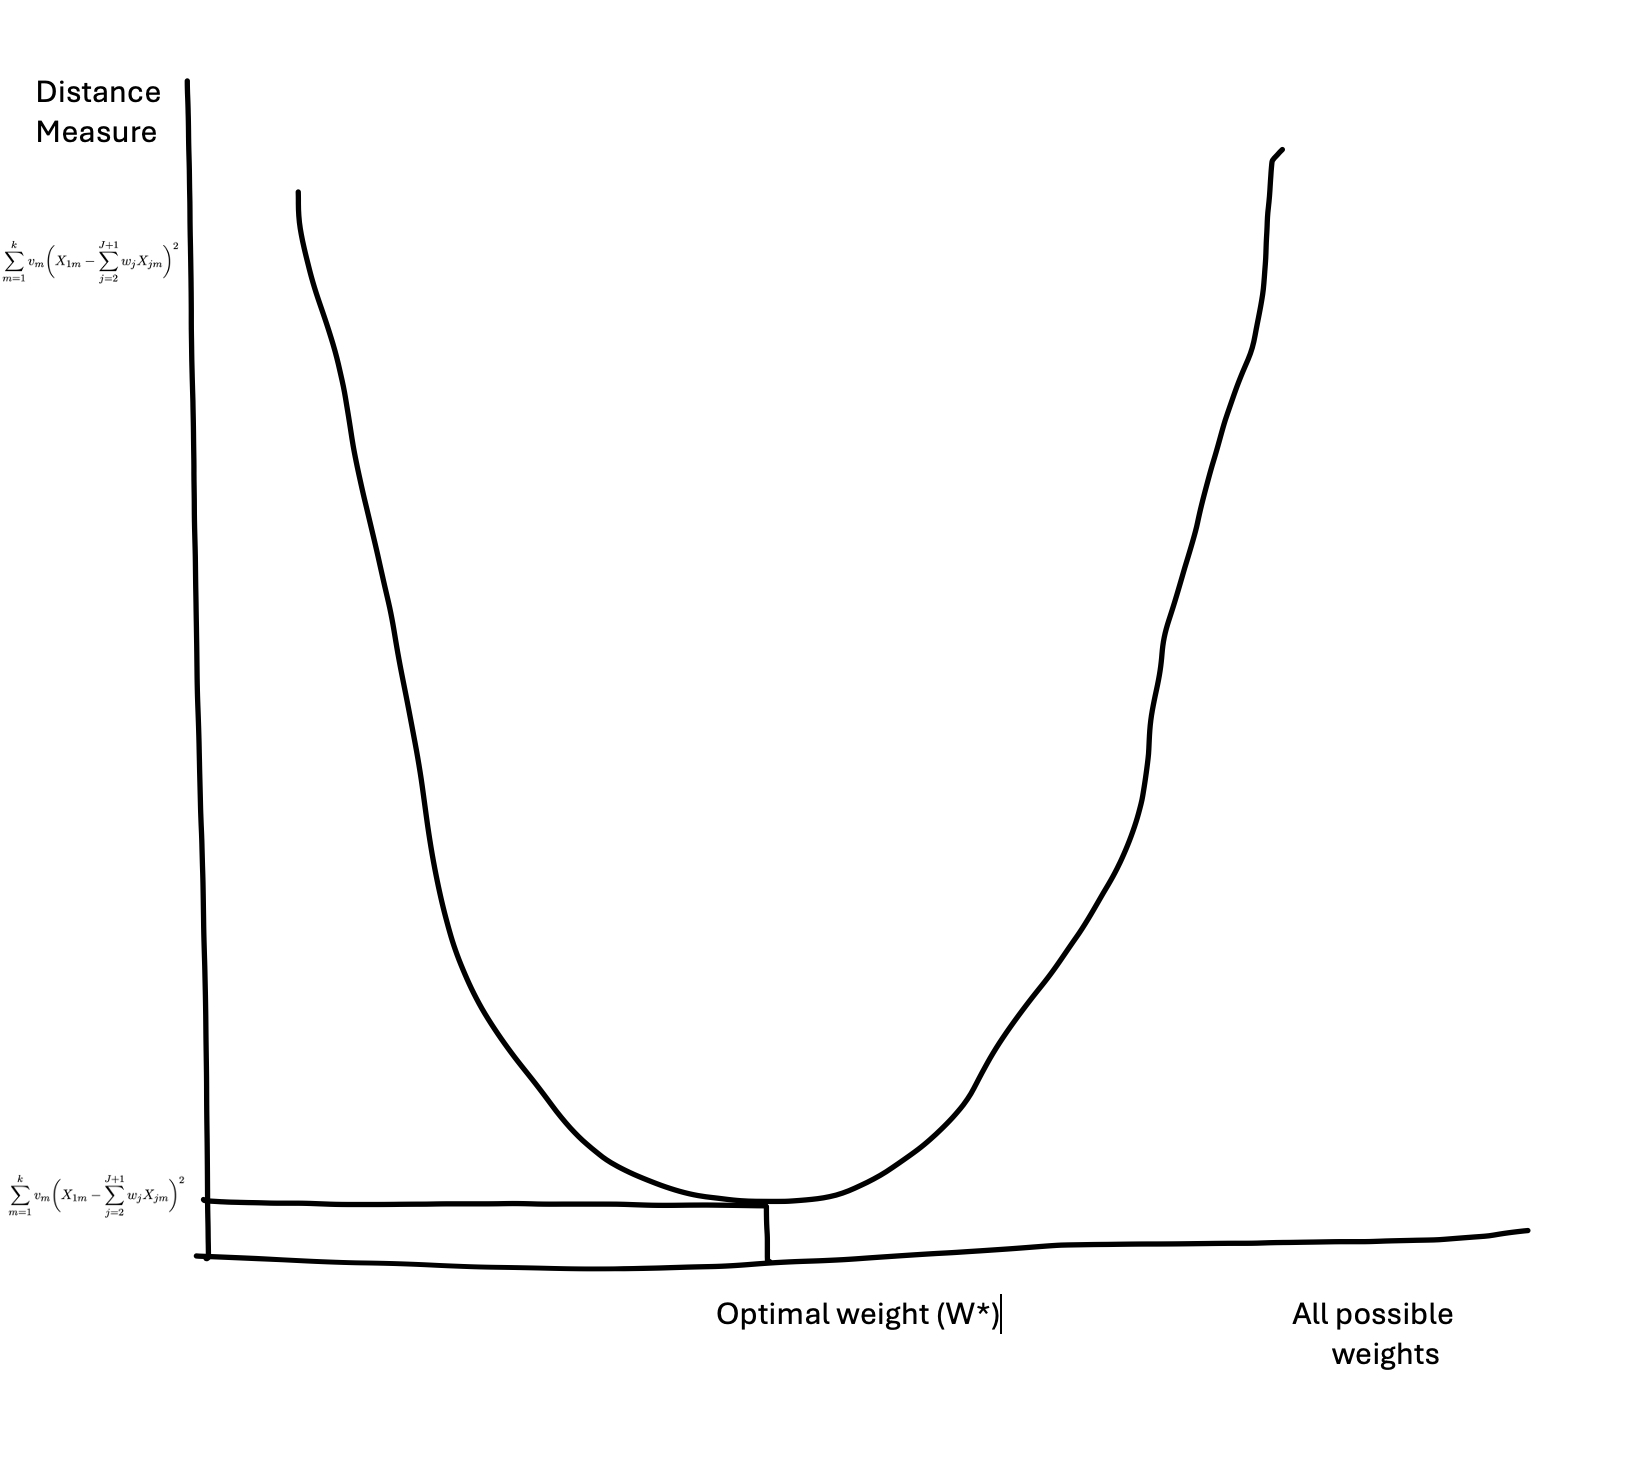
\includegraphics[scale=0.25]{./lecture_includes/synth_optimal_weight}
\end{figure}

\end{frame}



\begin{frame}{More on the V matrix}

Typically, $V$ is diagonal with main diagonal $v_1, \dots, v_k$.  Then, the synthetic control weights $w_2^*, \dots, w_{J+1}^*$ minimize: $$\sum_{m=1}^k v_m \bigg(X_{1m} - \sum_{j=2}^{J+1}w_jX_{jm}\bigg)^2$$ where $v_m$ is a weight that reflects the relative importance that we assign to the $m$-th variable when we measure the discrepancy between the treated unit and the synthetic controls

\end{frame}

\begin{frame}{Choice of $V$ is critical}
	
		\begin{itemize}
		\item The synthetic control $W^*(V^*)$ is meant to reproduce the behavior of the outcome variable for the treated unit in the absence of the treatment
		\item Therefore, the $V^*$ weights directly shape $W^*$
		\end{itemize}
\end{frame}

\begin{frame}{Estimating the $V$ matrix}
	
 Choice of $v_1, \dots, v_k$ can be based on
		\begin{itemize}
		\item Assess the predictive power of the covariates using regression
		\item Subjectively assess the predictive power of each of the covariates, or calibration inspecting how different values for $v_1, \dots, v_k$ affect the discrepancies between the treated unit and the synthetic control
		\item Minimize mean square prediction error (MSPE) for the pre-treatment period (default):
			\begin{eqnarray*}
			\sum_{t=1}^{T_0} \bigg(Y_{1t} - \sum_{j=2}^J w_j^*(V^*)Y_{jt} \bigg)^2
			\end{eqnarray*}
		\end{itemize}
\end{frame}

\begin{frame}{Cross validation}

\begin{itemize}
		\item Abadie recommends cross validation for selecting the covariates
		\item Divide the pre-treatment period into an initial \textbf{training} period and a subsequent \textbf{validation} period
		\item For any given $V$, calculate $W^*(V)$ in the training period.
		\item Minimize the MSPE of $W^*(V)$ in the validation period
\end{itemize}

\bigskip

Let's look at an example from the 2010 JASA paper with Hainmueller and Diamond

\end{frame}



\begin{frame}{Example: California's Proposition 99}
	
	\begin{itemize}
	\item In 1988, California first passed comprehensive tobacco control legislation:
		\begin{itemize}
		\item increased cigarette tax by 25 cents/pack
		\item earmarked tax revenues to health and anti-smoking budgets
		\item funded anti-smoking media campaigns
		\item spurred clean-air ordinances throughout the state
		\item produced more than \$100 million per year in anti-tobacco projects
		\end{itemize}
	\item Other states that subsequently passed control programs are excluded from donor pool of controls (AK, AZ, FL, HI, MA, MD, MI, NJ, OR, WA, DC)
	\end{itemize}
\end{frame}

\begin{frame}{Cigarette Consumption: CA and the Rest of the US}
	
	\begin{figure}
	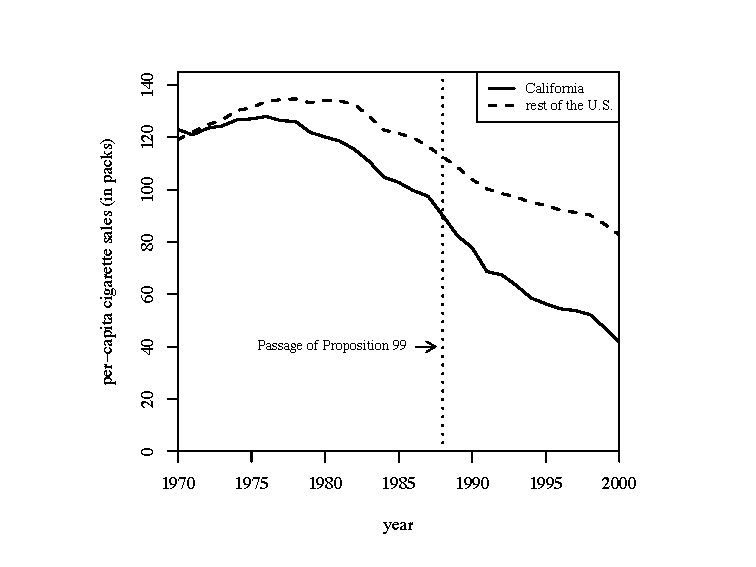
\includegraphics[scale=0.75]{./lecture_includes/abadie_3.pdf}
	\end{figure}
\end{frame}

\begin{frame}{Cigarette Consumption: CA and synthetic CA}
	
	\begin{figure}
	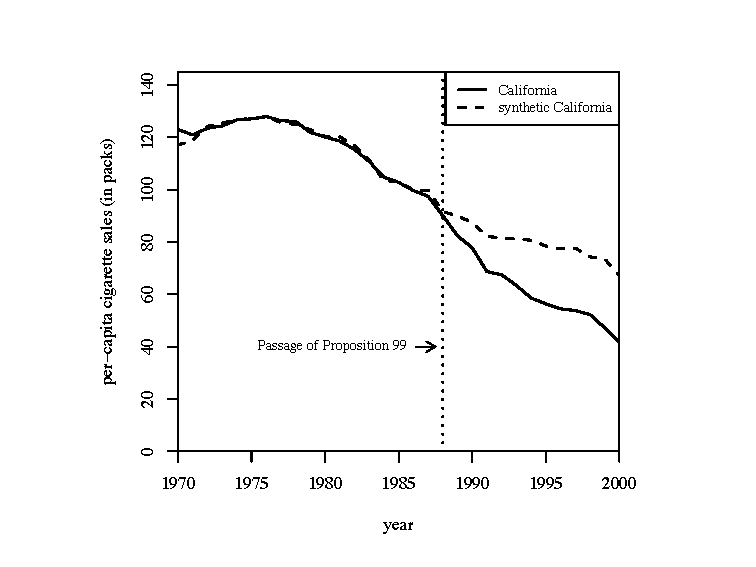
\includegraphics[scale=0.75]{./lecture_includes/abadie_4.pdf}
	\end{figure}
\end{frame}

\begin{frame}{Sparsity and Synthetic Control Weights}
	\begin{figure}
	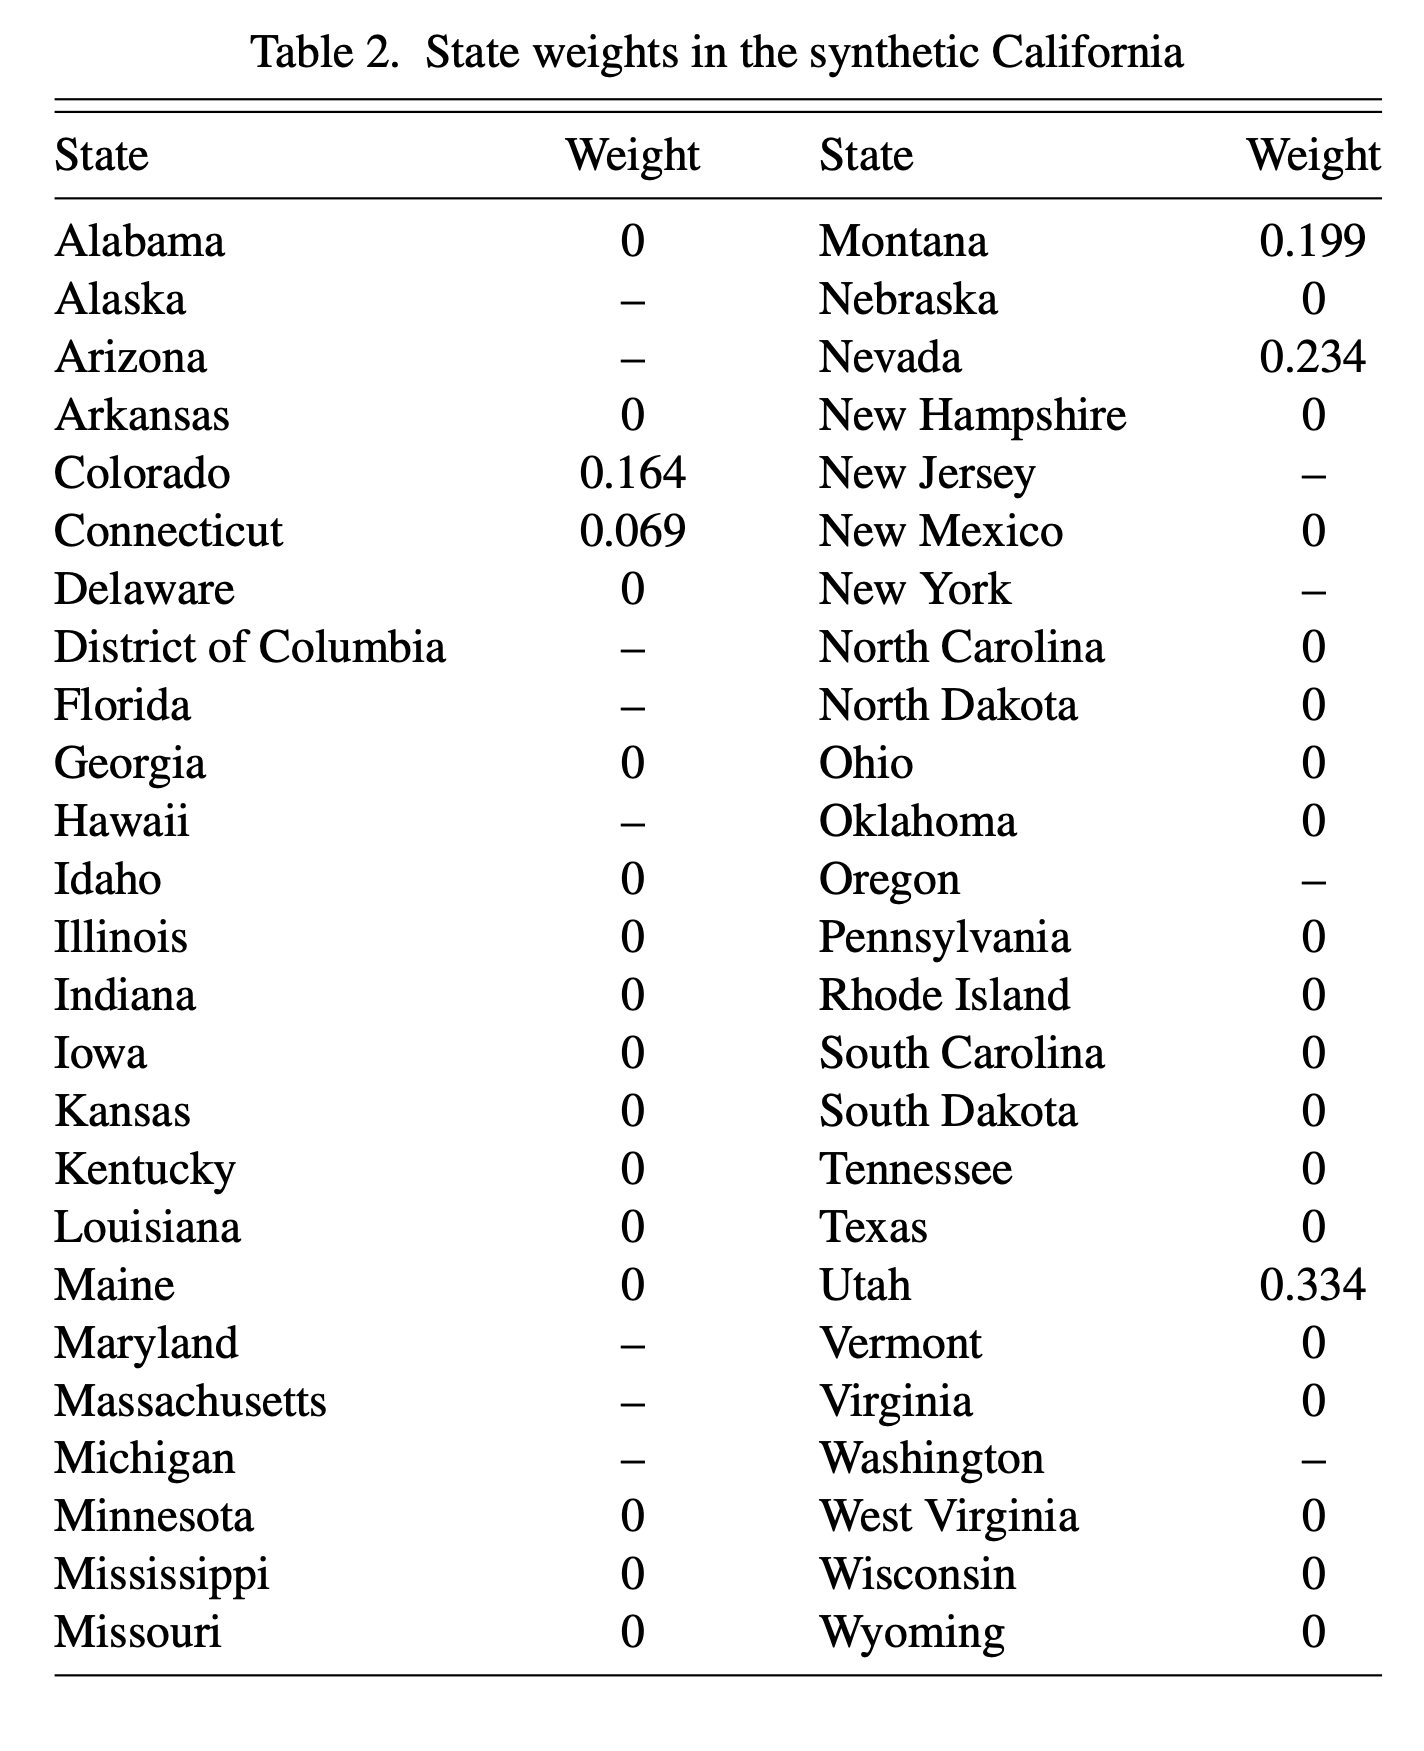
\includegraphics[scale=0.25]{./lecture_includes/synth_smoking_table2.png}
	\end{figure}
\end{frame}



\begin{frame}{Predictor Means: Actual vs. Synthetic California}
	
	\begin{figure}
	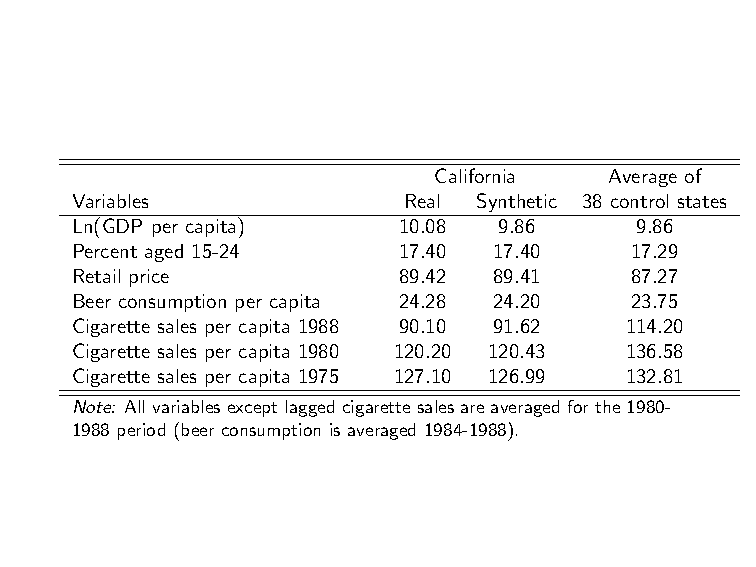
\includegraphics[scale=0.75]{./lecture_includes/abadie_5.pdf}
	\end{figure}
\end{frame}

\begin{frame}{Smoking Gap between CA and synthetic CA}
	
	\begin{figure}
	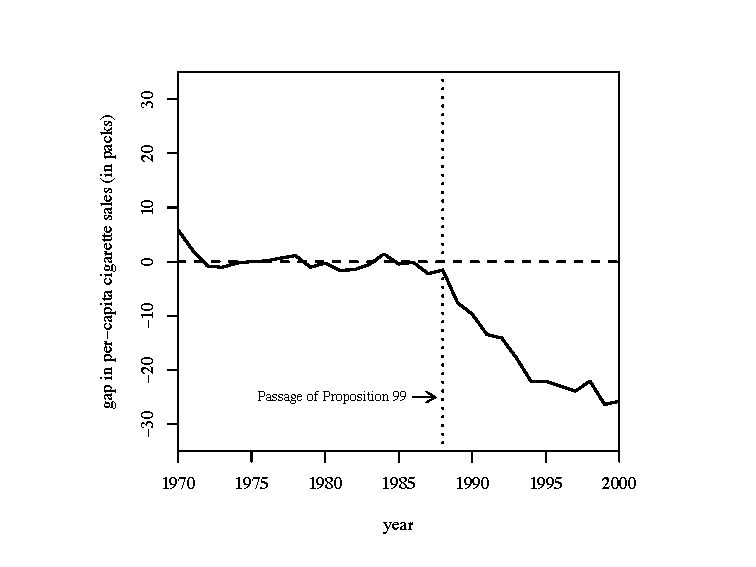
\includegraphics[scale=0.75]{./lecture_includes/abadie_6.pdf}
	\end{figure}
\end{frame}

\begin{frame}{Inference}
	
	\begin{itemize}
	\item To assess significance, we calculate exact p-values under Fisher's sharp null using a test statistic equal to after to before ratio of RMSPE
	\item Exact p-value method
		\begin{itemize}
		\item Iteratively apply the synthetic method to each country/state in the donor pool and obtain a distribution of placebo effects
		\item Compare the gap (RMSPE) for California to the distribution of the placebo gaps. For example the post-Prop. 99 RMSPE is: 
			\begin{eqnarray*}
			RMSPE = \bigg(\frac{1}{T-T_0} \sum_{t=T_0+1}^T \bigg(Y_{1t} - \sum_{j=2}^{J+1} w_j^* Y_{jt}\bigg)^2 \bigg)^{\frac{1}{2}}
			\end{eqnarray*}and the exact p-value is the treatment unit rank divided by $J$
		\end{itemize}
	\end{itemize}
\end{frame}

\begin{frame}{Smoking Gap for CA and 38 control states}
	
	\begin{figure}
	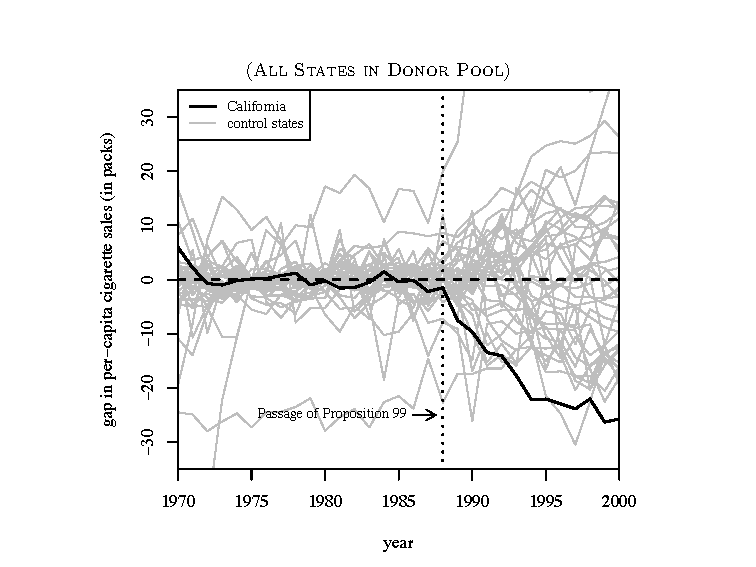
\includegraphics[scale=0.75]{./lecture_includes/abadie_7.pdf}
	\end{figure}
\end{frame}

\begin{frame}{Smoking Gap for CA and 34 control states}
	
	\begin{figure}
	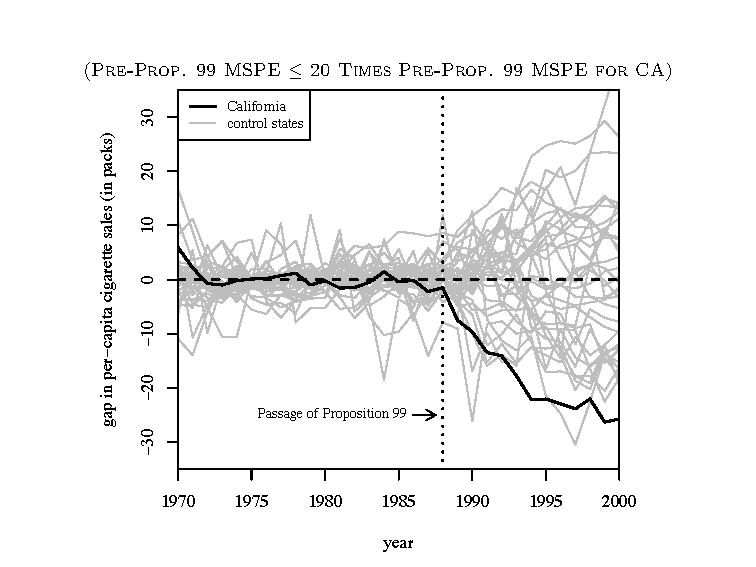
\includegraphics[scale=0.75]{./lecture_includes/abadie_8.pdf}
	\end{figure}
\end{frame}

\begin{frame}{Smoking Gap for CA and 29 control states}
	
	\begin{figure}
	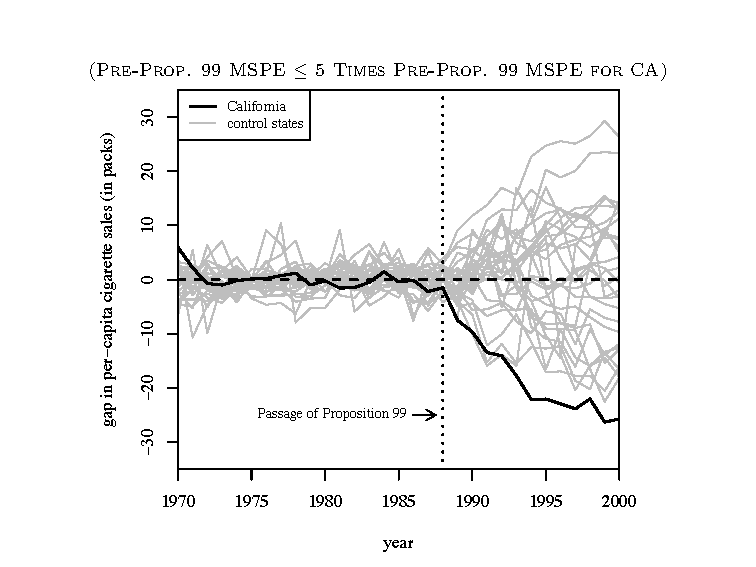
\includegraphics[scale=0.75]{./lecture_includes/abadie_9.pdf}
	\end{figure}
\end{frame}

\begin{frame}{Smoking Gap for CA and 19 control states}
	
	\begin{figure}
	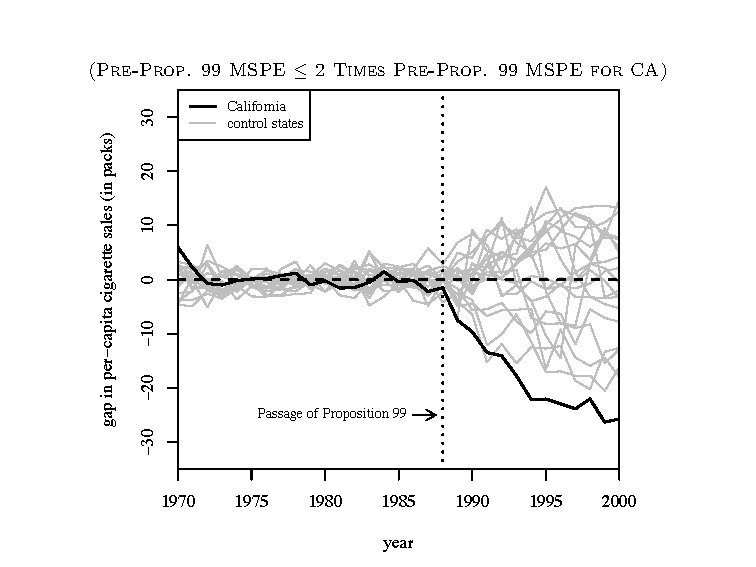
\includegraphics[scale=0.75]{./lecture_includes/abadie_10.pdf}
	\end{figure}
\end{frame}

\begin{frame}{Ratio Post-Prop. 99 RMSPE to Pre-Prop. 99 RMSPE}

	\begin{figure}
	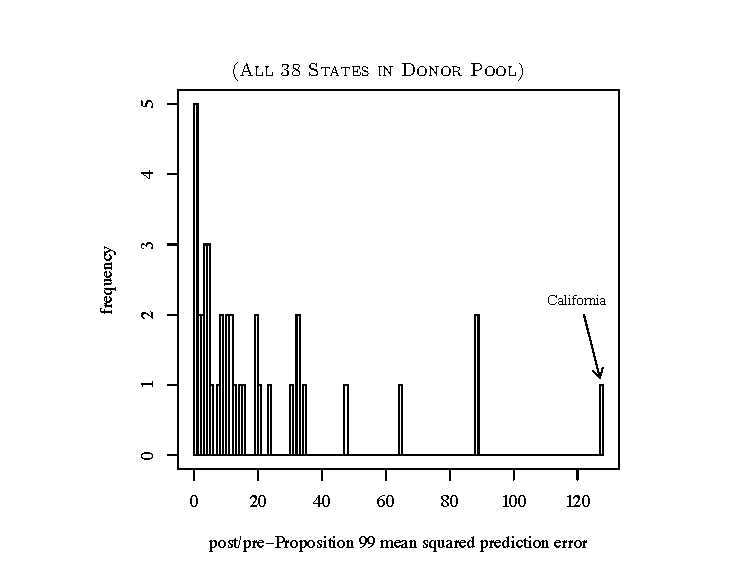
\includegraphics[scale=0.75]{./lecture_includes/abadie_11.pdf}
	\end{figure}
\end{frame}




\begin{frame}{Replication exercise}
	
	\begin{itemize}
	\item The US has the highest prison population of any OECD country in the world 
	\item 2.1 million are currently incarcerated in US federal and state prisons and county jails
	\item Another 4.75 million are on parole
	\item From the early 1970s to the present, incarceration and prison admission rates quintupled in size
	\end{itemize}
\end{frame}



\begin{frame}[plain]

\begin{figure}
\includegraphics[scale=0.5]{./lecture_includes/cook2010.pdf}
\end{figure}
\end{frame}


\begin{frame}{Prison constraints}

	
	\begin{itemize}
	\item Prisons are and have been at capacity for a long time so growth in imprisonment would bite on state corrections
	\item Managing increased flows can only be solved by the following:
		\begin{itemize}
		\item Prison construction
		\item Overcrowding
		\item Paroles
		\end{itemize}
	\item Texas chooses overcrowding
	\end{itemize}
\end{frame}



\begin{frame}{Ruiz v. Estelle 1980}

	
	\begin{itemize}
		\item Class action lawsuit against TX Dept of Corrections (Estelle, warden). 
		\item TDC lost.  Lengthy period of appeals and legal decrees.  
		\item Lengthy period of time relying on paroles to manage flows
	\end{itemize}
\end{frame}

\begin{frame}[plain]
  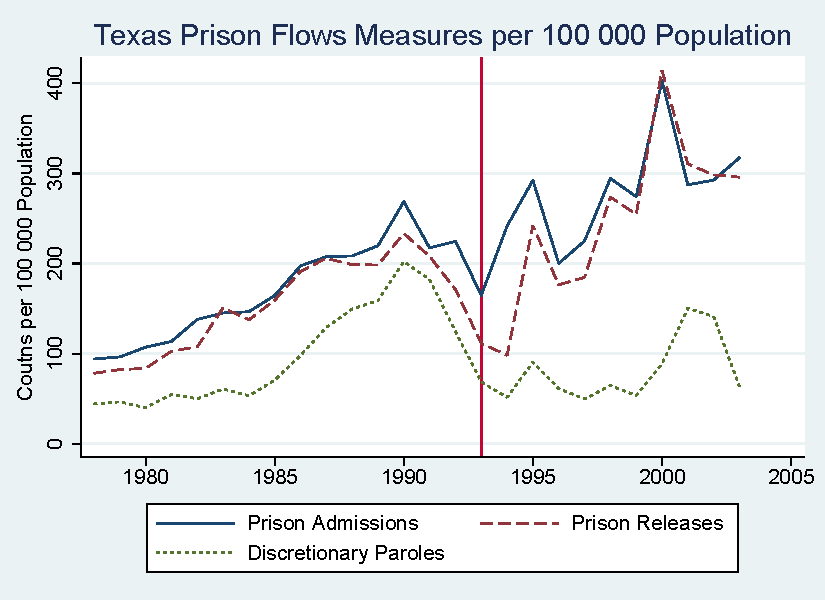
\includegraphics[scale=0.8]{./lecture_includes/flow_rate_figure.pdf}
\end{frame}

\begin{frame}{Texas prison boom}

Governor Ann Richards (D) 1991-1995
		\begin{itemize}
		\item Operation prison capacity increased 30-35\% in 1993, 1994 and 1995. 
		\item Prison capacity increased from 55,000 in 1992 to 130,000 in 1995.  
		\item Building of new prisons (private and public)
		\end{itemize} 
\end{frame}


\begin{frame}[shrink=30,plain]

\begin{figure}
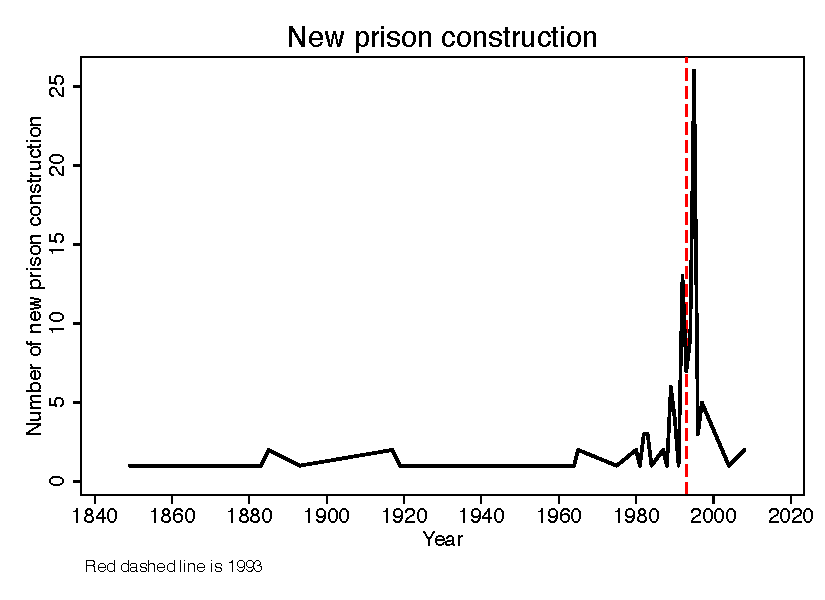
\includegraphics{./lecture_includes/tdcj.pdf}
\end{figure}
\end{frame}


\begin{frame}[shrink=30,plain]
\begin{figure}
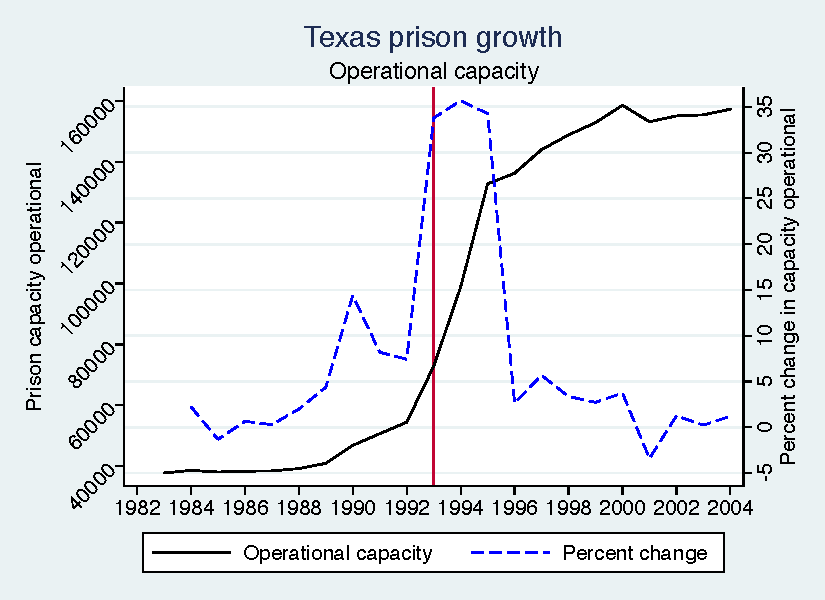
\includegraphics{./lecture_includes/capacity_operational_texas.pdf}
\end{figure}
\end{frame}



\begin{frame}[shrink=30,plain]

\begin{figure}
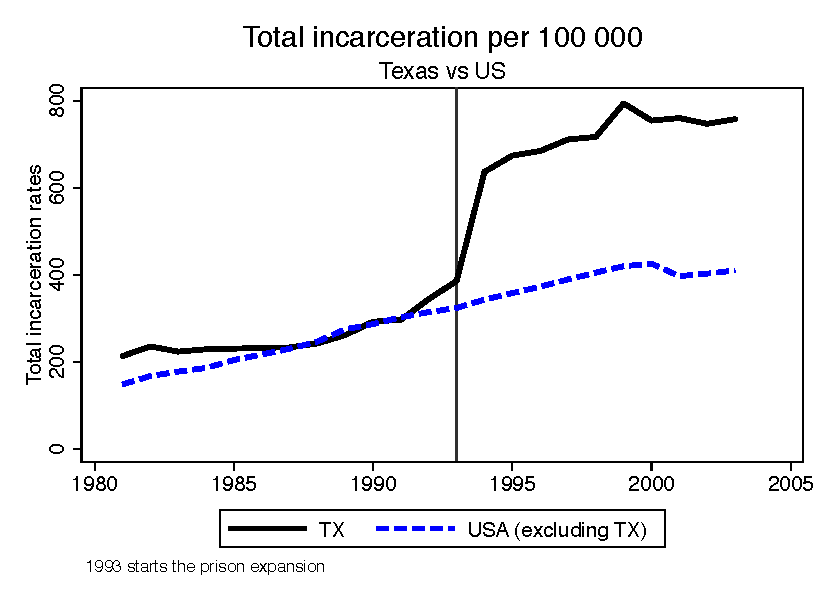
\includegraphics{./lecture_includes/total_incarceration.pdf}
\end{figure}
\end{frame}

\begin{frame}[shrink=30,plain]

\begin{figure}
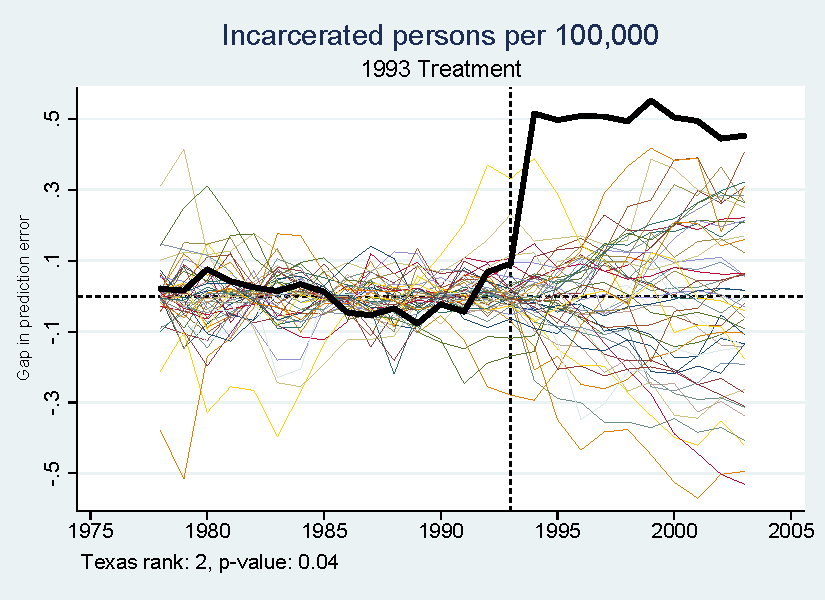
\includegraphics{./lecture_includes/synth_placebo_totalincarceration1993.pdf}
\end{figure}
\end{frame}


\begin{frame}{Coding together}

\begin{itemize}
\item Let's go to Mixtape Sessions repository now into /Labs/Texas 
\item I'll walk us through the Stata and R code so you understand the syntax and underlying logic
\item But then I have us a practice assignment 
\end{itemize}

\end{frame}


\begin{frame}{Summarizing}

\begin{itemize}

\item Method is simple: take donor pool units and find a combination of units, weight them, that minimize a distance function subject to two weight constraints $W*$ and $V*$.
\item But what is the bias and what can we do when we think the bias is severe?
\item We now move towards that now by examining the nature of the bias in synthetic control
\end{itemize}

\end{frame}




\subsection{Augmented Synthetic Control}


\begin{frame}{Imperfect Fit}

\begin{quote}
``The applicability of the [ADH2010] method requires a sizable number of pre-intervention periods. The reason is that the credibility of a synthetic control depends upon how well it tracks the treated unit’s characteristics and outcomes over an extended period of time prior to the treatment. \textbf{We do not recommend using this method when the pretreatment fit is poor or the number of pretreatment periods is small}. A sizable number of post-intervention periods may also be required in cases when the effect of the intervention emerges gradually after the intervention or changes over time.'' (my emphasis, Abadie, et al. 2015)
\end{quote}

\end{frame}




\begin{frame}{Augmenting synthetic control}

\begin{enumerate}
\item[1. ] Original synthetic control needs perfect fit and so will be biased in practical settings as it won't be the case we get weights constrained to be  on the convex hull
\item[2. ] Augmentation of the synthetic control estimator uses an outcome model to estimate the bias caused by covariate imbalance 
\item[3. ] Outcome model is a penalized ridge regression which will provide new weights we use to reweight the original synthetic control (bias adjustment in the spirit of Abadie and Imbens (2011)
\end{enumerate}

\end{frame}


\begin{frame}{Augmenting synthetic control}

\begin{enumerate}
\item[4. ] When synth is imbalanced, augmented synth will reduce bias reweighting and bias correction, and when synth is balanced, they are the same
\item[5. ] When synth is balanced, the augmented and original synth are identical (but in practice, they won't be identical)
\item[6. ] They argue synth DiD can be seen as a special case of augmented synth
\end{enumerate}

\end{frame}





\begin{frame}{Notation}

\begin{itemize}
\item Observe $J+1$ units over $T$ time periods
\item Unit $1$ will be treated at time period $T_0=T-1$ (we allow for unit $1$ to be an average over treated units)
\item Units $j=2 $ to $J+1$ (using ADH original notation) are ``never treated''
\item $D_j$ is the treatment indicator
\end{itemize}

\end{frame}



\begin{frame}{Optimal weights}

Synth minimizes the following norm:

\begin{eqnarray*}
\textrm{min}_w = || V_X^{1/2} (X_1 - X_0'w) ||_2^2 + \psi \sum_{D_j=0}f(w_j)\\
\textrm{s.t. }\sum_{j=2}^N w_{j} =1 \textrm{ and } w_j \geq 0
\end{eqnarray*}

$Y_0'w*$ (i.e., optimally weighted donor pool) is the unit 1 ``synthetic control'' 

\end{frame}


\begin{frame}{Predicting counterfactuals}

Synth minimizes the following norm:

\begin{eqnarray*}
\textrm{min}_w = || V_X^{1/2} (X_1 - X_0'w) ||_2^2 + \psi \sum_{D_j=0}f(w_j)\\
\textrm{s.t. }\sum_{j=2}^N w_{j} =1 \textrm{ and } w_j \geq 0
\end{eqnarray*}

We are hoping that $\widehat{Y}_1^0$ with $Y_0' {w}^{*}$ based on ``perfect fit'' pre-treatment

\end{frame}




\begin{frame}{Penalizing the weights with ridge}

Synth minimizes the following norm:

\begin{eqnarray*}
\textrm{min}_w = || V_X^{1/2} (X_1 - X_0'w) ||_2^2 + \psi \sum_{D_j=0}f(w_j)\\
\textrm{s.t. }\sum_{j=2}^N w_{j} =1 \textrm{ and } w_j \geq 0
\end{eqnarray*}

Modification to the original synthetic control model is the inclusion of the penalty term. ``The choice of penalty is less central when weights are constrained to be on the simplex, but becomes more important when we relax this constraint.''

\end{frame}

\begin{frame}{Convex hull}

Synth minimizes the following norm:

\begin{eqnarray*}
\textrm{min}_w = || V_X^{1/2} (X_1 - X_0'w) ||_2^2 + \psi \sum_{D_j=0}f(w_j)\\
\textrm{s.t. }\sum_{j=2}^N w_{j} =1 \textrm{ and } w_j \geq 0
\end{eqnarray*}

These weights will be used to address imbalance, not so much the control units, bc this method is for when the weighted controls are still outside the convex hull

\end{frame}




\begin{frame}{Original ADH factor model and bias}

\begin{eqnarray*}
Y_{it}^0 = \alpha_t + \theta_t Z_i + \lambda_t u_i + \varepsilon_{it}
\end{eqnarray*}

\bigskip

Original synth factor model (with ADH notation)

\bigskip

\begin{eqnarray*}
Y^0_{1t} - \sum^{J+1}_{j=2}w^*_jY_{jt} &=& \sum_{j=2}^{J+1} w_j^* \sum_{s=1}^{T_0} \lambda_t \bigg ( \sum_{n=1}^{T_0} \lambda_n'\lambda_n \bigg )
^{-1} \lambda_s'(\varepsilon_{js} - \varepsilon_{1s} ) \\
&& - \sum_{j=2}^{J+1} w_j^* (\varepsilon_{jt} - \varepsilon_{1t})
\end{eqnarray*}

\bigskip

The bias of ADH synthetic control


\end{frame}




\begin{frame}{Perfect fit is necessary}

\begin{eqnarray*}
Y^0_{1t} - \sum^{J+1}_{j=2}w^*_jY_{jt} &=& \sum_{j=2}^{J+1} w_j^* \sum_{s=1}^{T_0} \lambda_t \bigg ( \sum_{n=1}^{T_0} \lambda_n'\lambda_n \bigg )
^{-1} \lambda_s'(\varepsilon_{js} - \varepsilon_{1s} ) \\
&& - \sum_{j=2}^{J+1} w_j^* (\varepsilon_{jt} - \varepsilon_{1t})
\end{eqnarray*}

\bigskip

Recall that the bias of ADH required ``perfect fit'' using their factor model (I'll change $\lambda$ factor loadings in a minute)

\end{frame}




\begin{frame}{Perfect fit models heterogeneity}


\begin{eqnarray*}
Y^0_{1t} - \sum^{J+1}_{j=2}w^*_jY_{jt} &=& \sum_{j=2}^{J+1} w_j^* \sum_{s=1}^{T_0} \lambda_t \bigg ( \sum_{n=1}^{T_0} \lambda_n'\lambda_n \bigg )
^{-1} \lambda_s'(\varepsilon_{js} - \varepsilon_{1s} ) \\
&& - \sum_{j=2}^{J+1} w_j^* (\varepsilon_{jt} - \varepsilon_{1t})
\end{eqnarray*}

Only units that are alike in observables and unobservables should produce similar trajectories of the outcome variable over extended periods of time


\end{frame}



\begin{frame}{Slight change in synth notation}

\begin{itemize}
\item Assume that our outcome, $Y^0_{jt}$, follows a factor model where $m(.)$ are pre-treatment potential outcomes: $$ Y_{jt}^0 = m_{jt} + \varepsilon_{jt}$$
\item Since $\widehat{m(.)}$ estimates the post-treatment outcome, it can be viewed as an estimate of matching bias
\item Procedure then becomes analogous to bias correction for inexact matching (Abadie and Imbens 2011)
\end{itemize}

\end{frame}



\begin{frame}{Bias correction}

 $$ Y_{jt}^0 = m_{jt} + \varepsilon_{jt}$$

\begin{itemize}
\item Recall from earlier by Abadie, et al. (2010) and Ferman and Pinto (2021) the same point made which is that as $T$ grows, the synthetic control achieves balance, not by fitting on the idiosyncratic noise (which is on average zero in large samples), but on the unobserved heterogeneity in the factor model
\item Thus when the weights do achieve exact balance, the bias of synthetic control decreases with $T$
\end{itemize}

\end{frame}



\begin{frame}{Common practice}

\begin{itemize}
\item Usually the number of time periods isn't much larger than the number of units
\item And exact balance rarely holds, which if it doesn't hold, then the unobserved heterogeneity also doesn't get deleted even with large $T$
\end{itemize}

\end{frame}

\begin{frame}{Estimating the bias}

\begin{itemize}
\item Adjust the synthetic control to adjust for poor fit pre-treatment with an estimate of the ``matching bias'' for both the treatment group and the weighted average donor pools (Abadie and Imbens 2011)
\item We will use our outcome regression model, $\widehat{m}_{jT}$, to estimate the post-treatment potential outcome $Y_{jT}^0$ which is recall unobserved for treatment group
\item So there is in other words two steps involved: estimate the synthetic control finding optimal donor pool weights, then estimate the matching bias using ridge regression and adjust, similar to bias correction in Abadie and Imbens 2011
\end{itemize}


\end{frame}




\begin{frame}{Setup of the estimator}

$Y_1^{aug,0}$ is the augmented potential outcome based on synthetic control (first term) and adjustments for matching imbalance (second and third terms):

\begin{eqnarray*}
Y_1^{aug,0} &=& \sum_{D_j=0} \widehat{w}_j^{synth} Y_{j} + \widehat{m}(X_1) - \sum_{D_j=0} \widehat{w}_j \widehat{m}(X_j) \\
&=& \widehat{m}(X_1) + \sum_{D_j=0} \widehat{w_j}(Y_j - \widehat{m}(X_j))
\end{eqnarray*}

\end{frame}


\begin{frame}{Interpreting line 1}

\begin{eqnarray*}
Y_1^{aug,0} &=& \sum_{D_j=0} \widehat{w}_j^{synth} Y_{jT} + \bigg (\widehat{m}_{1T} - \sum_{D_j=0} \widehat{w}_j^{synth}\widehat{m}_{jT} \bigg ) \\
&=& \widehat{m}_{1T} + \sum_{D_j=0} \widehat{w}_j^{synth} (Y_{jT} - \widehat{m}_{jT})
\end{eqnarray*}

(1) Note how in the first line the traditional synthetic control weighted outcomes are corrected by the imbalance in a particular function of the pre-treatment outcomes $\widehat{m}$. 
\end{frame}




\begin{frame}{Interpreting line 1}

\begin{eqnarray*}
Y_1^{aug,0}  &=& \sum_{D_j=0} \widehat{w}_j^{synth} Y_{jT} + \bigg (\widehat{m}_{1T} - \sum_{D_j=0} \widehat{w}_j^{synth}\widehat{m}_{jT} \bigg ) \\
&=& \widehat{m}_{1T} + \sum_{D_j=0} \widehat{w}_j^{synth} (Y_{jT} - \widehat{m}_{jT})
\end{eqnarray*}

(1) Since $\widehat{m}$ estimates the post-treatment outcome, we can view this as an estimate of the bias due to imbalance, which is similar to how you address imbalance in matching with a bias correction formula (Abadie and Imbens 2011). 

\end{frame}




\begin{frame}{Interpreting line 1}
\begin{eqnarray*}
Y_1^{aug,0}  &=& \sum_{D_j=0} \widehat{w}_j^{synth} Y_{jT} + \bigg (\widehat{m}_{1T} - \sum_{D_j=0} \widehat{w}_j^{synth}\widehat{m}_{jT} \bigg ) \\
&=& \widehat{m}_{1T} + \sum_{D_j=0} \widehat{w}_j^{synth} (Y_{jT} - \widehat{m}_{jT})
\end{eqnarray*}

(1) So if the bias is small, then synthetic control and augmented synthetic control will be similar because that interior term will be zero.

\end{frame}

\begin{frame}{Interpreting line 2}

\begin{eqnarray*}
Y_1^{aug,0}  &=& \sum_{D_j=0} \widehat{w}_j^{synth} Y_{jT} + \bigg (\widehat{m}_{1T} - \sum_{D_j=0} \widehat{w}_j^{synth}\widehat{m}_{jT} \bigg ) \\
&=& \widehat{m}_{1T} + \sum_{D_j=0} \widehat{w}_j^{synth} (Y_{jT} - \widehat{m}_{jT})
\end{eqnarray*}

(2) The second line is a double robust representation of the estimator equal to a regression based outcome model plus weighted residuals


\end{frame}

\begin{frame}{Form of outcome model}

\begin{itemize}

\item To estimate $\widehat{m}$, recall it is an extrapolation of $Y^0$ based on covariates $X$ (ignoring subscripts)
\item But this can have overfitting problems, so they introduce a ridge regression
\item Issue will be with regards to the hyperparameter so they'll suggest cross validation
\item It's inside this second ``reweighting'' stage (or bias adjustment) that the negative weighting comes and it comes from the outcome model itself extrapolating

\end{itemize}

\end{frame}




\begin{frame}{Ridge Augmented SCM}

\begin{eqnarray*}
\textrm{arg min}_{\eta_0,\eta} \frac{1}{2} \sum_{D_j=0} (Y_j - (\eta_0 + X_j'\eta))^2 + \lambda^{ridge} || \eta ||_2^2
\end{eqnarray*}Here we estimate $\widehat{m}(X_j)$ with ridge regularized linear model and penalty hyper parameter $\lambda^{ridge}$. Sorry -- this is not the same $\lambda$. I didn't create this notation though! Once we have those, we adjust for imbalance using the $\widehat{\eta}^{ridge}$ parameter as a weight on the outcome model itself. 

\end{frame}

\begin{frame}{Ridge Augmented SCM}

\begin{eqnarray*}
\textrm{arg min}_{\eta_0,\eta} \frac{1}{2} \sum_{D_j=0} (Y_j - (\eta_0 + X_j'\eta))^2 + \lambda^{ridge} || \eta ||_2^2
\end{eqnarray*}Once we have those, we adjust for imbalance using the $\widehat{\eta}^{ridge}$ parameter as a weight on the outcome model itself. 

\end{frame}




\begin{frame}{Go back to that weighting but use the ridge parameters}

\begin{eqnarray*}
Y_1^{aug,0} &=& \sum_{D_j=0} \widehat{w}_j^{synth} Y_{j} + \bigg ( X_1 - \sum_{D_j=0} \widehat{w}_j^{synth} X_j \bigg ) \widehat{\eta}^{ridge} \\
&=& \sum_{D_j=0} \widehat{w}_j^{aug}Y_j
\end{eqnarray*}What you're trying to do is adjust with the $\widehat{w}_j^{aug}$ weights to improve balance.  

\end{frame}


\begin{frame}{The ridge weights are key to the augmentation}

\begin{eqnarray*}
\widehat{w}_j^{aug} = \widehat{w}_j^{synth} + (X_j - X_0' \widehat{w}_j^{synth}) ' (X_0'X_0 + \lambda I_{T_0})^{-1}X_i
\end{eqnarray*}

The second term is adjusting the original synthetic control weights, $w_j^{synth}$ for better balance. Again remember -- we are trying to address the bias due to imbalance. You can achieve better balance, but at higher variance and can introduce negative weights. 

\end{frame}



\begin{frame}{Ridge will allow negative weights via extrapolation}

\begin{eqnarray*}
\widehat{w}_j^{aug} = \widehat{w}_j^{synth} + (X_j - X_0' \widehat{w}_j^{synth}) ' (X_0'X_0 + \lambda I_{T_0})^{-1}X_i
\end{eqnarray*}

Relaxing the constraint from synth that weights be non-negative, as non-negative weights prohibit extrapolation. But we don't have synthetic control on the simplex, so we \emph{must} extrapolate, otherwise synth will be biased.

\end{frame}



\begin{frame}{Summarizing and some comments}

\begin{itemize}
\item When the treated unit lies in the convex hull of the control units so that the synth weights exactly balance lagged outcomes, then SCM and Ridge ASCM are the same
\item When synth weights do not achieve exact balance, Ridge ASCM will use negative weights to extrapolate from the convex hull to the control units
\item The amount of extrapolation will be determined by how much imbalance we're talking about and the estimated hyperparameter $\widehat{\lambda}^{ridge}$
\item When synth has good pre-treatment fit or when $\lambda^{ridge}$ is large, then adjustment will be small and the augmented weights will be close to the SCM weights
\end{itemize}

\end{frame}




\begin{frame}{Augmented synth vs original synthetic control}

\begin{itemize}
\item In conclusion, synthetic control is best when pre-treatment fit is excellent, otherwise it is biased
\item Synthetic control avoids extrapolation by restricting weights to be non-negative and sum to one
\item Ridge regression augmentation will allow for a degree of extrapolation to achieve pre-treatment balance and that creates negative weights
\item Augmented synth will dominate synth in those instances by extrapolating outside the convex hull
\end{itemize}

\end{frame}





\begin{frame}{Replication}

\begin{itemize}
\item We will now show code that does it in R and Stata
	\begin{itemize}
	\item R: "augsynth" by the authors
	\item Stata: "allsynth" that does several (including augsynth)
	\end{itemize}
\item Two examples to hopefully illustrate the bias and improvements and the lack of bias and no change in another
	\begin{itemize}
	\item Smoking: augmented synth improves it
	\item Prisons: augmented synth does nothing
	\end{itemize}
\end{itemize}

\end{frame}






\subsection{Synthetic difference-in-differences}

\begin{frame}
\frametitle{The Basic Idea of SDID}

\begin{itemize}
    \item Combines ideas from synthetic control and difference-in-differences.
        \begin{itemize}
            \item Matches control units to treated units with pre-treatment weights.
            \item Addresses biases from imperfect matching.
        \end{itemize}
    \item Introduces time weights to prioritize key pre-treatment periods.
    \item Balances precision from synthetic control with broader trends from DID.
\end{itemize}

\end{frame}

\begin{frame}
\frametitle{How SDID Works}

\begin{itemize}
    \item Uses unit and time fixed effects for bias reduction.
        \begin{itemize}
            \item Accounts for unit-specific traits (e.g., state-level differences).
            \item Captures common period effects (e.g., economic booms).
        \end{itemize}
    \item Derives time weights directly from the data.
    \item Flexible tool for causal inference in complex panel data.
\end{itemize}

\end{frame}

\begin{frame}
\frametitle{Intuition Behind SDID}

\begin{itemize}
    \item Approximates parallel trends by reweighting data.
        \begin{itemize}
            \item Unit weights align control and treated units pre-treatment.
            \item Time weights balance trends across periods.
        \end{itemize}
    \item Reduces reliance on strong assumptions about pre-existing trends.
    \item Enhances robustness when pre-existing trends don’t align perfectly.
\end{itemize}

\end{frame}


\begin{frame}
\frametitle{Assumptions in Synthetic Difference-in-Differences (SDID)}

In both synthetic control and difference-in-differences, assumptions about pre-treatment trends are central. SDID combines these methods to leverage their strengths:

\begin{itemize}
    \item Uses pre-treatment trends to reweight treated and control groups.
    \item Constructs a comparison group that mimics the treated group's trends.
    \item Relies on four key assumptions for identification.
\end{itemize}

\end{frame}


\begin{frame}
\frametitle{Assumption 1: Error Properties}

\begin{itemize}
    \item Errors are independent, identically distributed Gaussian vectors.
    \item Covariance matrix has bounded eigenvalues.
    \item Assumption is stricter than traditional DiD or synthetic control, which only assume error independence.
\end{itemize}

\end{frame}


\begin{frame}
\frametitle{Assumption 2: Sample Sizes}

\begin{itemize}
    \item Large sample sizes are critical for SDID:
    \begin{itemize}
        \item Number of control units ($N_{co}$) and pre-treatment periods ($T_{pre}$) must be large.
        \item Product of treated units ($N_{tr}$) and post-treatment periods ($T_{post}$) should also be large.
    \end{itemize}
    \item Balance between $T_{pre}$ and $N_{co}$ ensures effective reweighting.
\end{itemize}

\end{frame}


\begin{frame}
\frametitle{Assumptions 3 and 4}

\textbf{Assumption 3: Systematic Component Properties}
\begin{itemize}
    \item The systematic component ($L$) has a limited number of large singular values.
    \item This low-rank structure captures broad patterns while reducing noise.
    \item Goes beyond traditional DiD and synthetic control.
\end{itemize}

\vspace{0.5cm}

\textbf{Assumption 4: Weighting Properties and $L$}
\begin{itemize}
    \item "Oracle" weights derived from $L$ reduce systematic bias.
    \item Ensures parallel trends after reweighting without requiring perfect balance.
\end{itemize}

\end{frame}






\begin{frame}
\frametitle{Steps in SDID Estimation}

\begin{itemize}
    \item Identify unit weights for control units to match treated pre-treatment trends.
    \item Select time weights to balance pre- and post-treatment trends.
    \item Combine weights in regression to estimate the ATT.
\end{itemize}

\end{frame}



\begin{frame}
\frametitle{SDID Estimation Process}

\begin{itemize}
    \item Calculates unit and time weights to optimize comparison groups.
    \item Uses regularization to prevent overfitting.
        \begin{itemize}
            \item Aligns with one-period outcome changes for untreated units.
        \end{itemize}
    \item Solves constrained least-squares for unit weights (\(\hat{w}\)).
\end{itemize}

\end{frame}

\begin{frame}{Estimation of SDiD}

Synthetic DiD combines elements of DiD and synthetic control:
\begin{itemize}
    \item Compute the regularization parameter to align with typical one-period outcome changes:
    \[
    \Delta_{it} = Y_{i(t+1)} - Y_{it} \quad \text{(unexposed units)}.
    \]
\end{itemize}

\end{frame}





\begin{frame}
\frametitle{Unit and Time Weights}

\begin{itemize}
    \item \textbf{Unit Weights (\(\hat{w}\)):}
        \begin{itemize}
            \item Match treated and control units pre-treatment.
            \item Allows for a constant gap, relaxing traditional SC constraints.
        \end{itemize}
    \item \textbf{Time Weights (\(\hat{\lambda}\)):}
        \begin{itemize}
            \item Balance temporal dynamics.
            \item Prioritize informative pre-treatment periods.
        \end{itemize}
\end{itemize}

\end{frame}


\begin{frame}{Estimating Weights}

\begin{itemize}
    \item Unit Weights:
    \begin{itemize}
        \item Estimated via constrained least squares on pre-treatment data.
        \item Weights are non-negative, sum to one, and allow for a level shift with regularization.
    \end{itemize}
    \item Time Weights:
    \begin{itemize}
        \item Estimated via constrained least squares on control data.
        \item Prioritizes periods just before treatment without spreading weights broadly.
    \end{itemize}
\end{itemize}

\end{frame}



\begin{frame}{Estimation of SDiD: Unit Weights}

\begin{itemize}
    \item Estimate unit weights \(\widehat{w}\) to define a synthetic control unit.
    \item Equation: 
    \[
    \widehat{w}_1 + \widehat{w}^T Y_{j,\text{pre}} \approx Y_{1,\text{pre}}
    \]
    \item Unlike traditional synthetic control, allows for an intercept term, relaxing perfect matching requirements.
\end{itemize}

\end{frame}

\begin{frame}{Estimation of SDiD: Time Weights}

\begin{itemize}
    \item Estimate time weights \(\widehat{\lambda}\) to align synthetic pre-treatment periods:
    \[
    \widehat{\lambda}_1 + Y_{1,\text{pre}} \widehat{\lambda} \approx Y_{1,\text{post}}
    \]
    \item Focuses on identifying pre-treatment periods most informative for post-treatment behavior.
\end{itemize}

\end{frame}



\begin{frame}
\frametitle{Combined Estimation}

\begin{itemize}
    \item SDID estimator combines unit and time weights.
    \item Weighted regression minimizes residuals across units and time.
    \item Ensures counterfactual outcomes align with treated outcomes pre-treatment.
\end{itemize}

\end{frame}




\begin{frame}
\frametitle{Outcome Model in SDID}

\begin{itemize}
    \item Observed outcomes (\(Y\)) consist of:
        \begin{itemize}
            \item Systematic component (\(L\)).
            \item Treatment effect (\(D \circ \delta\)).
            \item Idiosyncratic error (\(E\)).
        \end{itemize}
    \item \(D \circ \delta\) isolates ATT by selecting treated units and periods.
    \item \(L\) captures trends not explained by treatment or noise.
\end{itemize}

\end{frame}




\begin{frame}
\frametitle{Oracle Weights}

\begin{itemize}
    \item Theoretical "ideal" weights for unit (\(\tilde{\omega}\)) and time (\(\tilde{\lambda}\)).
    \item Minimize bias by balancing systematic component (\(L\)).
    \item Data-driven weights (\(\hat{\omega}, \hat{\lambda}\)) approximate oracle weights.
        \begin{itemize}
            \item Ensure pre-treatment balance.
            \item Converge to oracle weights as sample size increases.
        \end{itemize}
\end{itemize}

\end{frame}



\begin{frame}{Outcome Model}
\begin{itemize}
\item Outcome is a combination of systematic trends, treatment effects, and noise:
\[
Y = L + D \circ \delta + E
\]
\item Components:
    \begin{itemize}
    \item \(L\): systematic trends across units and time (\(L = \Gamma \Upsilon^\top\))
    \item \(D \circ \delta\): treatment effects applied selectively
    \item \(E\): idiosyncratic noise
    \end{itemize}
\item \(L\) represents shared patterns unaffected by treatment or randomness.
\end{itemize}
\end{frame}

\begin{frame}{Role of Systematic Component \(L\)}
\begin{itemize}
\item Captures trends unrelated to treatment or random noise.
\item Potential source of confounding if not properly controlled.
\item Treated and control groups must balance \(L\) pre-treatment for valid comparison.
\end{itemize}
\end{frame}

\begin{frame}{Oracle Weights}
\begin{itemize}
\item Theoretical weights (\(\tilde{\omega}, \tilde{\lambda}\)) minimize bias in estimating treatment effects.
\item Balance systematic trends (\(L\)) across treated and control groups.
\item Provide a benchmark for robust causal inference.
\end{itemize}
\end{frame}

\begin{frame}{Data-Driven Weights}
\begin{itemize}
\item Empirical weights (\(\hat{\omega}, \hat{\lambda}\)) approximate oracle weights.
\item Constructed to balance treated and control trends pre-treatment.
\item Approximation improves with larger sample sizes.
\end{itemize}
\end{frame}

\begin{frame}{Weighted Regression for SDiD}

\begin{itemize}
    \item Final estimation uses weighted DID regression:
\end{itemize}

\[
\textrm{argmin}_{\tau, \mu, \alpha, \beta} \sum_{i=1}^N \sum_{t=1}^T \left( Y_{it} - \mu - \alpha_i - \beta_t - W_{it}\tau \right)^2 \widehat{w}_i^{\text{SDiD}} \widehat{\lambda_t}^{\text{SDiD}}
\]

\end{frame}




\begin{frame}{Regression Comparison: SC, DiD, SDiD}

\begin{itemize}
    \item Synthetic Control (SC):
    \[
    \tau^{\text{SC}} = \textrm{argmin}_{\tau, \lambda} \sum_{i,t} (Y_{it} - \lambda_t - \tau D_{it})^2 w_i^{\text{SC}}
    \]
    \item Difference-in-Differences (DiD):
    \[
    \textrm{argmin}_{\tau, \lambda, \alpha} \sum_{i,t} (Y_{it} - \lambda_t - \alpha_i - \tau D_{it})^2
    \]
    \item Synthetic Difference-in-Differences (SDiD):
    \[
    \textrm{argmin}_{\tau, \lambda, \alpha} \sum_{i,t} (Y_{it} - \lambda_t - \alpha_i - \tau D_{it})^2 w_i \lambda_t
    \]
\end{itemize}

\end{frame}

\begin{frame}{Key Features of SDiD}

\begin{itemize}
    \item Combines synthetic control's matching with DID's parallel trends adjustment.
    \item Introduces unit and time weights for improved balance.
    \item Does not require perfect pre-treatment matching or strictly parallel trends.
\end{itemize}

\end{frame}




\begin{frame}{Decomposing the Bias of SDiD}
\[
\widehat{\tau}^{sdid} - \tau = \varepsilon(\widetilde{w}, \widetilde{\lambda}) + B(\widetilde{w}, \widetilde{\lambda}) + \widehat{\tau}(\widehat{w},\widehat{\lambda}) - \widehat{\tau}(\widetilde{w},\widetilde{\lambda})
\]
\begin{itemize}
\item \textbf{Oracle noise}: Variance introduced by weights and sample limitations.
\item \textbf{Oracle confounding bias}: Systematic differences not removed by weights.
\item \textbf{Deviation from oracle}: Approximation errors in empirical weights.
\end{itemize}
\end{frame}

\begin{frame}{Oracle Noise}
\begin{itemize}
\item Noise arises from random variation in data.
\item Small when weights (\(\hat{w}, \hat{\lambda}\)) are small and sample sizes are sufficient.
\item Ensures noise does not dominate the estimator.
\end{itemize}
\end{frame}

\begin{frame}{Oracle Confounding Bias: Units and Time}
\begin{itemize}
\item \textbf{Units (Rows)}:
    \[
    \widetilde{w_1} + \widetilde{w_{j}}^TL_{j,pre} \approx \widetilde{w}_1^TL_{1,pre}
    \]
    \[
    \widetilde{w_1} + \widetilde{w_{j}}^TL_{j,post} \approx \widetilde{w}_1^TL_{1,post}
    \]
    Ensures weights remove bias from systematic differences across units.
\item \textbf{Time (Columns)}:
    \[
    \widetilde{\lambda_1} + \widetilde{\lambda_{j}}^TL_{j,pre} \approx \widetilde{\lambda}_1^TL_{1,pre}
    \]
    \[
    \widetilde{\lambda_1} + \widetilde{\lambda_{j}}^TL_{j,post} \approx \widetilde{\lambda}_1^TL_{1,post}
    \]
    Captures temporal dynamics to align treated and control groups.
\end{itemize}
\end{frame}

\begin{frame}{Doubly Robust Property}
\begin{itemize}
\item Sufficient for one set of weights (unit or time) to generalize well.
\item Combination of oracle unit and time weights can compensate for failures in one dimension.
\item Provides resilience against systematic confounding.
\end{itemize}
\end{frame}

\begin{frame}{Deviation from Oracle}
\begin{itemize}
\item SDID approximates oracle weights when:
    \begin{itemize}
    \item Oracle weights generalize well on training sets.
    \item Regularization is appropriately tuned.
    \end{itemize}
\item Ensures SDID estimator is close to theoretical benchmark.
\end{itemize}
\end{frame}


\begin{frame}
\frametitle{Practical Implications}

\begin{itemize}
    \item Combines theoretical rigor with empirical flexibility.
    \item Balances systematic trends in pre-treatment data.
    \item Achieves robust causal inference for ATT estimation.
\end{itemize}

\end{frame}



\begin{frame}{Practical Considerations: Pre-treatment Trends}

\begin{itemize}
    \item Visually inspect pre-treatment trends to check for alignment between treated and control groups.
    \item Use plots to ensure parallel trends are approximately valid before treatment.
    \item Address any unusual patterns or discrepancies early.
\end{itemize}

\end{frame}


\begin{frame}{Practical Considerations: Weights and Assumptions}

\begin{itemize}
    \item Balanced weights:
    \begin{itemize}
        \item Ensure $\hat{\omega}$ and $\hat{\lambda}$ are not overly concentrated.
        \item Adjust regularization parameters if needed.
    \end{itemize}
    \item Assess parallel trends:
    \begin{itemize}
        \item Contextual knowledge remains crucial.
        \item Account for potential confounders.
    \end{itemize}
\end{itemize}

\end{frame}


\begin{frame}{Practical Considerations: SEs and Heterogeneous Effects}

\begin{itemize}
    \item Standard errors:
    \begin{itemize}
        \item Select bootstrap or other approaches suited to your data structure.
        \item Be cautious with small treated samples.
    \end{itemize}
    \item Heterogeneous effects:
    \begin{itemize}
        \item Consider if ATT is the correct focus.
        \item Explore alternative approaches for widely varying effects.
    \end{itemize}
\end{itemize}

\end{frame}







\begin{frame}{Key Takeaway}

\begin{itemize}
    \item Synthetic DiD offers a practical, flexible, and robust approach for causal inference in complex panel data.
    \item Balances strengths of synthetic control and difference-in-differences while mitigating their weaknesses.
    \item Poised to become a valuable tool in causal panel analysis.
\end{itemize}

\end{frame}


\begin{frame}{Concluding Remarks: Synthesis of Methods}

\begin{itemize}
    \item Combines synthetic control (matching precision) with difference-in-differences (parallel trends).
    \item Addresses challenges in synthetic control’s convex hull constraint.
    \item Regularization allows for approximate matches with intercept terms.
\end{itemize}

\end{frame}






\begin{frame}{Concluding Remarks: Robustness and Applications}

\begin{itemize}
    \item Doubly robust:
    \begin{itemize}
        \item Performs well as long as unit or time weights succeed.
    \end{itemize}
    \item Adaptable to cases where:
    \begin{itemize}
        \item Diff-in-diff assumptions are weak.
        \item Synthetic control fit is imperfect.
    \end{itemize}
    \item Links to augmented synthetic control for two-way bias reduction.
\end{itemize}

\end{frame}




\begin{frame}{Practical Problems}
\begin{itemize}
\item \textbf{Underfitting}: Cannot achieve parallel pre-treatment trends.
    \begin{itemize}
    \item Solution: Explore more or better controls or alternative methods.
    \end{itemize}
\item \textbf{Omitted Variable Bias}: External factors coincide with treatment, leading to identification failure.
\item \textbf{Overfitting}: Synthetic control perfectly matches pre-treatment but fails post-treatment.
    \begin{itemize}
    \item Analogous to RDD functional form issues.
    \end{itemize}
\end{itemize}
\end{frame}

\begin{frame}{How to Rule Out Overfitting: Oracle Weights}
\begin{itemize}
\item Estimator matches an "oracle" that avoids overfitting by design.
\item Oracle weights minimize expected squared error, not just in-sample error.
\item Weights are robust to noise in the data.
\end{itemize}
\end{frame}


\begin{frame}{Properties of SDID}
\begin{itemize}
\item Approximately unbiased and normally distributed under large samples.
\item Optimal variance, estimable via clustered bootstrap.
\item Robust to noise and systematic confounding.
\end{itemize}
\end{frame}






\begin{frame}{R code: synthdid}

Let's look at the code together

\bigskip

Code: \url{https://github.com/synth-inference/synthdid} 

\bigskip

Vignettes: \url{https://synth-inference.github.io/synthdid/articles/more-plotting.html}

\end{frame}




\begin{frame}{Abadie on the value and use of synthetic control}

	\begin{figure}
	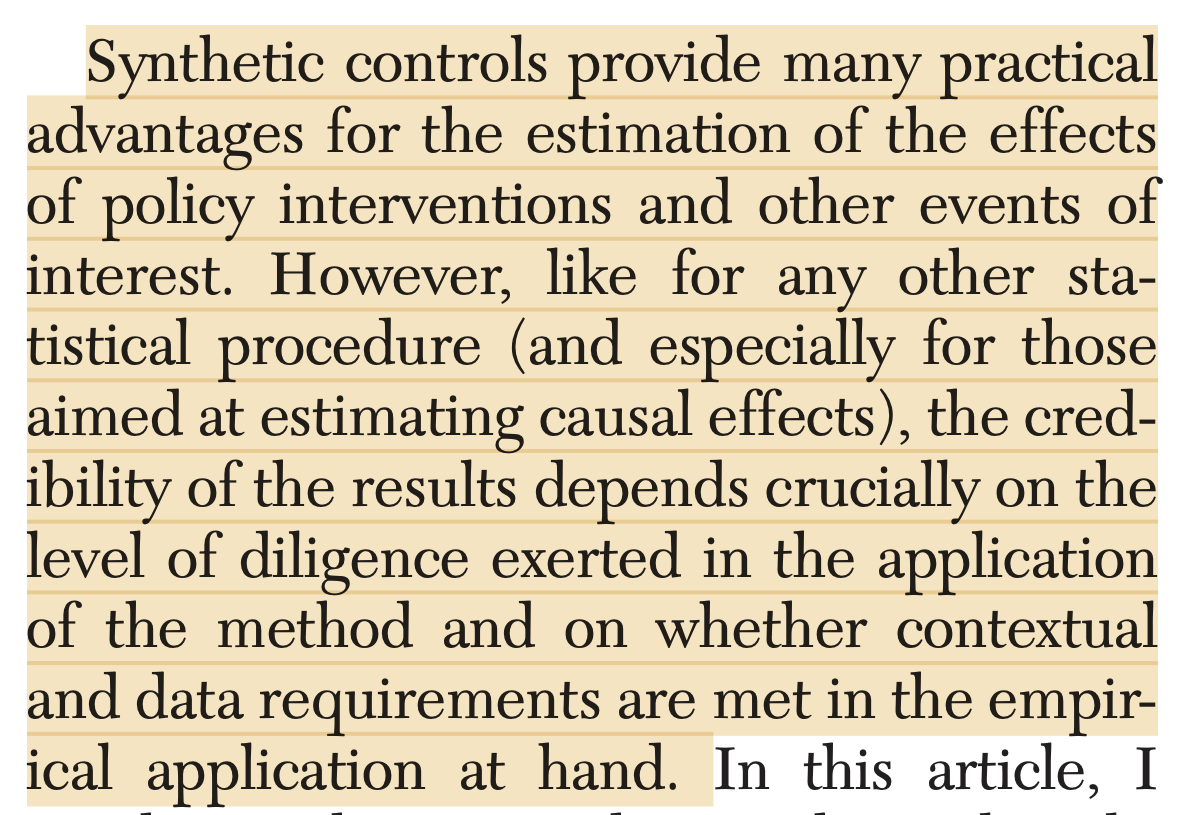
\includegraphics[scale=0.5]{./lecture_includes/abadie_quote.png}
	\end{figure}

\end{frame}


\begin{frame}{Summarizing}


\begin{itemize}

\item Synthetic control was developed for the comparative case study; it is a kind of matching estimator with an underlying factor model for its identification (not parallel trends)
\item Advancements have been made along multiple dimensions -- bias adjustments, demeaning, as well as exploring more general structures than just factor models
\item It is now a more robust, general causal panel method but the assumptions needed to justify it need "due diligence" 

\end{itemize}

\end{frame}

\begin{frame}{Closing remark}

\begin{itemize}
\item Focus on the treatment assignment mechanisms carefully to help understand how unobserved time varying confounders may be threatening your results, pay close attention to issues around observable matching bias, remember the importance of the "long panel"
\item Extrapolation based on the negative weighting should be done with the idea of bias reduction (augmented ridge), not simply for the purpose of fitting
\item Good luck!

\end{itemize}

\end{frame}




\end{document}